\documentclass[addpoints]{exam}
\usepackage{preamble}
\sisetup{group-separator = {,}}
%\extrawidth{-3in} %Use for pasting questions in PowerPoint

\pagestyle{headandfoot}
\runningheadrule

\firstpagefooter{Access for free at \href{https://openstax.org/books/astronomy-2e/pages/1-introduction}{https://openstax.org/books/astronomy-2e/pages/1-introduction}}{}{}
\runningfooter{Access for free at \href{https://openstax.org/books/astronomy-2e/pages/1-introduction}{https://openstax.org/books/astronomy-2e/pages/1-introduction}}{}{}

\firstpageheader{Astronomy}{Checks For Understanding}{Chapter 2: {\small Observing the Sky}}

\CorrectChoiceEmphasis{\color{red}\bfseries}
\SolutionEmphasis{\color{red}}
%\printanswers

\begin{document}
\begin{questions}

\section*{2.1 The Sky Above}

\question
Imagine you are standing outside. Describe a way you can figure out the four cardinal directions (N, S, E, W) without the aid of a compass or technology.

\begin{solution}
    The place where the Sun rises is (approximately) East. Face East and extend your arms out to the side, like a cross. North is to your left, South to your right, and West behind you.

    Alternatively, if at night, you can locate the North Star using your knowledge of the positions of constellations, and repeat a similar exercise to the one described above.
\end{solution}

\begin{EnvUplevel}
\textbf{See the figure below and answer questions \ref{ques:CelestialSphere_start} through \ref{ques:CelestialSphere_end}.}
\end{EnvUplevel}

\begin{figure}[h!]
    \centering
\begin{tikzpicture}
\def\R{2.5} % sphere radius
\def\angEl{10} % elevation angle
\def\angBeta{25} % latitude of point P and Q


\pgfmathsetmacro\H{\R*cos(\angEl)} % distance to north pole
\node at (-0.2,0.7) {\small \textbf{E}};
\shade[ball color=white,opacity=0.5] (0,0) circle (\R);
\coordinate[mark coordinate] (O) at (0,0);

\begin{scope}[rotate=30]
    \DrawLatitudeCircleBack[\R]{0}
\end{scope}

\FillLatitudeCircle[\R]{0}
\DrawLatitudeCircle[\R]{0}

\draw[->] (0,0.15*\R) -- (0,1.01*\R) node[above] {\framebox{\textbf{A}}};

\begin{scope}[rotate=30]
    \draw[thick] (0,\R) -- (0,\R*1.25) node[left=1pt,align=left] {\framebox{\textbf{B}}} (0,-\R) -- (0,-\R*1.25) node[right=1pt,align=left] {\framebox{\textbf{C}}};
    \draw[dashed,very thin] (0,\R) -- (0,0.2) (0,-0.22*\R) -- (0,-\R);
    \DrawLatitudeCircleFront[\R]{0}
\end{scope}

\draw[red] (-\R*0.7,-\R*0.52) --++ (-\R*0.2,-\R*0.3) node[below left,align=left] {\color{red}\textbf{Celestial Equator}};
\node[left] at (-\R,0) {\textbf{N}};
\node[right] at (\R,0) {\textbf{S}};
\draw (2,0.25) -- ++(1,0.7) node[right] {\framebox{\textbf{D}}};

\node at (0,0.1) {\Strichmaxerl[1.8]};
\node at (0.8*\R,0.9*\R) {\framebox{\textbf{E}}};
\node at (0.1,-\R*0.3) {\textbf{W}};
\end{tikzpicture}
\end{figure}

\question \label{ques:CelestialSphere_start} 
What does \framebox{\textbf{D}} represent?

\begin{choices}
    \choice the celestial equator
    \correctchoice the horizon
    \choice the zenith
    \choice the constellations
\end{choices}

\question 
The surrounding ball, object \framebox{\textbf{E}}, is the \fillin\ .

\begin{choices}
    \choice ecliptic
    \choice celestial ellipsoid
    \choice cardinal point
    \correctchoice celestial sphere
\end{choices}

\question
Point \framebox{\textbf{A}} is the \fillin\ .

\begin{choices}
    \choice north celestial pole
    \choice celestial sphere
    \correctchoice zenith
    \choice ecliptic
\end{choices}

\question 
Which mark is the north celestial pole?

\begin{oneparchoices}
    \choice \framebox{\textbf{A}}
    \correctchoice \framebox{\textbf{B}}
    \choice \framebox{\textbf{C}}
    \choice \framebox{\textbf{D}}
    \choice \framebox{\textbf{E}}
\end{oneparchoices}

\question \label{ques:CelestialSphere_end} 
Point \framebox{\textbf{C}} is the \fillin .

\begin{choices}
    \choice north celestial pole
    \choice zenith
    \correctchoice south celestial pole
    \choice ecliptic
\end{choices}

\begin{solution}
    A distinct region of the sky, represented by a star pattern of a person or familiar shape. A ``comet in Orion'' means that the comet passed through the region of the sky bounded by the Orion constellation.
\end{solution}

\question
Suppose you are located somewhere on Earth where the celestial equator is oriented as shown below. What is your possible location?

\begin{minipage}{0.33\textwidth}
\begin{choices}
\choice Australia
\choice Ecuador
\choice The North Pole
\correctchoice California
\end{choices}
\end{minipage}%
\begin{minipage}{0.50\textwidth}
    \centering
\begin{tikzpicture}[scale=1,every node/.style={minimum size=1cm}]
\def\R{2} % sphere radius
\def\angEl{10} % elevation angle
\def\angBeta{45} % latitude of point P and Q

\node at (0.1,-\R*0.3) {\small \textbf{W}};
\pgfmathsetmacro\H{\R*cos(\angEl)} % distance to north pole
\node[left] at (0.38,0.67) {\small \textbf{E}};
\shade[ball color=white,opacity=0.5] (0,0) circle (\R);
\coordinate[mark coordinate] (O) at (0,0);


\begin{scope}[rotate=\angBeta]
    \DrawLatitudeCircleRedBack[\R]{0}
\end{scope}

\FillLatitudeCircle[\R]{0}
\DrawLatitudeCircle[\R]{0}

\draw[->] (0,0.15*\R) -- (0,\R) node[above=-8pt] {Zenith};

\begin{scope}[rotate=\angBeta]
    \DrawLatitudeCircleRedFront[\R]{0}
\end{scope}

\node[left] at (-\R*0.9,0) {\textbf{N}};
\node[right] at (\R*0.9,0) {\textbf{S}};

\draw (1.3,1) -- ++(1.2,0.8) node[right] {Celestial equator}; 

\node at (0,0.1) {\Strichmaxerl[1.8]};
\end{tikzpicture}
\end{minipage}%

\question
Suppose you are located somewhere on Earth where the celestial equator runs directly above you. What is your possible location?

\begin{minipage}{0.33\textwidth}
\begin{choices}
\choice Texas
\choice The North Pole
\choice South Africa
\correctchoice Ecuador 
\end{choices}
\end{minipage}%
\begin{minipage}{0.50\textwidth}
    \centering
\begin{tikzpicture}[scale=1,every node/.style={minimum size=1cm}]
\def\R{2} % sphere radius
\def\angEl{10} % elevation angle
\def\angBeta{25} % latitude of point P and Q

\node at (0.1,-\R*0.3) {\small \textbf{W}};
\pgfmathsetmacro\H{\R*cos(\angEl)} % distance to north pole
\node[left] at (0.38,0.67) {\small \textbf{E}};
\shade[ball color=white,opacity=0.5] (0,0) circle (\R);
\coordinate[mark coordinate] (O) at (0,0);

\begin{scope}[rotate=90]
    \DrawLatitudeCircleRedBack[\R]{0}
\end{scope}

\FillLatitudeCircle[\R]{0}
\DrawLatitudeCircle[\R]{0}

\draw[->] (0,0.15*\R) -- (0,\R) node[above=-8pt] {Zenith};

\begin{scope}[rotate=90]
    \DrawLatitudeCircleRedFront[\R]{0}
\end{scope}

\node[left] at (-\R*0.9,0) {\textbf{N}};
\node[right] at (\R*0.9,0) {\textbf{S}};

\draw (0.33,1) -- ++(1.2,0.8) node[right] {Celestial equator}; 

\node at (0,0.1) {\Strichmaxerl[1.8]};
\end{tikzpicture}
\end{minipage}

\question
Suppose you are located somewhere on Earth where the celestial equator is oriented as shown below. What is your possible location?

\begin{minipage}{0.33\textwidth}
\begin{choices}
\correctchoice Australia
\choice Texas
\choice Alaska
\choice Ecuador 
\end{choices}
\end{minipage}%
\begin{minipage}{0.50\textwidth}
    \centering
\begin{tikzpicture}[scale=1,every node/.style={minimum size=1cm}]
\def\R{2} % sphere radius
\def\angEl{10} % elevation angle
\def\angBeta{-45} % latitude of point P and Q

\node at (0.1,-\R*0.3) {\small \textbf{W}};
\pgfmathsetmacro\H{\R*cos(\angEl)} % distance to north pole
\node[left] at (0.38,0.67) {\small \textbf{E}};
\shade[ball color=white,opacity=0.5] (0,0) circle (\R);
\coordinate[mark coordinate] (O) at (0,0);


\begin{scope}[rotate=\angBeta]
    \DrawLatitudeCircleRedBack[\R]{0}
\end{scope}

\FillLatitudeCircle[\R]{0}
\DrawLatitudeCircle[\R]{0}

\draw[->] (0,0.15*\R) -- (0,\R) node[above=-8pt] {Zenith};

\begin{scope}[rotate=\angBeta]
    \DrawLatitudeCircleRedFront[\R]{0}
\end{scope}

\node[left] at (-\R*0.9,0) {\textbf{N}};
\node[right] at (\R*0.9,0) {\textbf{S}};

\draw (-1.3,1) -- ++(-1.2,0.8) node[left] {Celestial equator}; 

\node at (0,0.1) {\Strichmaxerl[1.8]};
\end{tikzpicture}
\end{minipage}%

\question %23. 
What is a \textbf{constellation} as astronomers define it today? What does it mean when an astronomer says, ``I saw a comet in Orion last night''?

\question %1 
From where on Earth could you observe all of the stars during the course of a year? 

\begin{solution}
The terrestrial equator. Use Stellarium to see this for yourself.
\end{solution}

\question
What fraction of the sky can be seen from the North Pole?

\begin{solution}
    Only half the sky.
\end{solution}



% \question %8 
% How many degrees does the Sun move per day relative to the fixed stars? How many days does it take for the Sun to return to its original location relative to the fixed stars?



\question %12 
Is the ecliptic the same thing as the celestial equator? Explain.

\begin{solution}
    No. Although there are both cicles on the celestial sphere, the ecliptic denotes the path the Sun will take on the celestial sphere across one year, and the celestial equator is the circle that divides the celestial sphere into norther and southern hemispheres. They are misaligned by \SI{23.5}{\degree} (see OpenStax Figure 2.7.)
\end{solution}


% \question %22 
% Describe a practical way to determine in which constellation the Sun is found at any time of the year.

\clearpage
\begin{EnvUplevel}
    \textbf{Consider the figure below. Then answer questions \ref{ques:Figure2.7_start} through \ref{ques:Figure2.7_end}.}
\end{EnvUplevel}


\begin{figure}[h!]
    \centering
\begin{tikzpicture}
\def\R{3} % sphere radius
\def\angEl{23} % elevation angle
\def\angTilt{30} %tilt angle increased from 23.5 for emphasis

\pgfmathsetmacro\H{\R*cos(\angEl)} % distance to north pole
\draw (0,0) -- (0,\H*1.25);
\draw[very thick,fill=yellow] (0.3,1.15) circle (3pt);%node[above right=-8pt] {\textbf{September}};

\begin{scope}[rotate=-\angTilt]
    \draw[very thin] (0,\H) -- (0,0);
\end{scope}
\shade[ball color=white,opacity=0.5] (0,0) circle (\R);
\coordinate[mark coordinate] (O) at (0,0);

\begin{scope}[rotate=-\angTilt]
    \DrawLatitudeCircleBack[\R]{0}
\end{scope}

\begin{scope}[rotate=-\angTilt]
        \DrawLatitudeCircleFront[\R]{0}
        \draw[thick] (0,\H*1.25) -- (0,\H) (0,0) -- (0,-1);
        \draw[very thick,blue,fill=white] (0,0) circle (19pt) node {\rotatebox{-\angTilt}{\textbf{Earth}}};
        \node at (0.2,0.9) {\textbf{N}};
        \node at (-0.2,-0.9) {\textbf{S}};
\end{scope}

\DrawLatitudeCircle[\R]{0}
\draw (-2,-0.9) --++ (-1.3,-0.6) node[left] {\framebox{\textbf{D}}};

\draw[very thick,fill=yellow] (-\R,0) circle (4pt);

\draw[very thick, fill=yellow] (\R,0) circle (4pt);
\draw (\R,0) -- ++ (1,1) node[right] {\framebox{\textbf{E}}};

\draw[very thick,fill=yellow] (-0.3,-1.15) circle (4pt);

\draw[very thick,<->] (0,2.3) arc (90:55:1.85);
\node at (0.7,2.6) {\framebox{\textbf{B}}};

\draw[thick] (1.7,-1.8) -- ++(1,-0.4) node[right] {\framebox{\textbf{A}}};

\node at (-1.05,0.2) {\framebox{\textbf{C}}};
\end{tikzpicture}
\end{figure}

\question \label{ques:Figure2.7_start} 
This figure represents a model that is \fillin\ .
\begin{choices}
\correctchoice geocentric
\choice heliocentric
\choice lunarcentric
\choice all of the above
\end{choices}

\question
Which figure label represents \textbf{Earth}?

\begin{oneparchoices}
    \choice \framebox{\textbf{A}}
    \choice \framebox{\textbf{B}}
    \correctchoice \framebox{\textbf{C}}
    \choice \framebox{\textbf{D}}
    \choice \framebox{\textbf{E}}
\end{oneparchoices}

\question
Which figure label represents the \textbf{celestial equator}?

\begin{oneparchoices}
    \correctchoice \framebox{\textbf{A}}
    \choice \framebox{\textbf{B}}
    \choice \framebox{\textbf{C}}
    \choice \framebox{\textbf{D}}
    \choice \framebox{\textbf{E}}
\end{oneparchoices}

\question
Which figure label represents the \textbf{Sun}?

\begin{oneparchoices}
    \choice \framebox{\textbf{A}}
    \choice \framebox{\textbf{B}}
    \choice \framebox{\textbf{C}}
    \choice \framebox{\textbf{D}}
    \correctchoice \framebox{\textbf{E}}
\end{oneparchoices}

\question 
Which figure label represents the \textbf{ecliptic}?

\begin{oneparchoices}
    \choice \framebox{\textbf{A}}
    \choice \framebox{\textbf{B}}
    \choice \framebox{\textbf{C}}
    \correctchoice \framebox{\textbf{D}}
    \choice \framebox{\textbf{E}}
\end{oneparchoices}


\question \label{ques:Figure2.7_end} 
Which figure label represents the \SI{23}{\degree} tilt of Earth's rotation relative to the ecliptic plane?

\begin{oneparchoices}
    \choice \framebox{\textbf{A}}
    \correctchoice \framebox{\textbf{B}}
    \choice \framebox{\textbf{C}}
    \choice \framebox{\textbf{D}}
    \choice \framebox{\textbf{E}}
\end{oneparchoices}


\question %10 
Explain how the zodiacal constellations are different from the other constellations.

\begin{solution}
    Zodiacal constellations align with the ecliptic, which is the circular path on the celestial sphere followed by the Sun throughout 1 year. Non-zodiacal constellations are not on the ecliptic.
\end{solution}


% \question %35. 
% What is the altitude of the north celestial pole in the sky from your latitude? If you do not know your latitude, look it up. If you are in the Southern Hemisphere, answer this question for the south celestial pole, since the north celestial pole is not visible from your location.


\clearpage
\section*{2.2 Ancient Astronomy}

\question %14 
Why did Pythagoras believe that Earth should be spherical?

\begin{solution}
    Because circles and spheres are ``perfect forms,'' and gods love them. Furthermore, Earth must be circular by extension of the observation that the Sun and Moon are circular.
\end{solution}

\question %15 
How did Aristotle deduce that the Sun is farther away from Earth than the Moon?

\begin{solution}
    He observed that the Moon sometimes get in front of the Sun, forming a solar eclipse. This can only happen if the Sun is behind the Moon.
\end{solution}

\question %16 
What are two ways in which Aristotle deduced that Earth is spherical?

\begin{solution}
    He observed that during a lunar eclipse Earth's shadow on the lunar surface is round. Second, he noticed that as one travels south the celestial shifts to expose new stars, feat which occurs on a round planet.
\end{solution}

\question %36. 
If you were to drive to some city south of your current location, how would the altitude of the celestial pole in the sky change?

\begin{solution}
    As Aristotle observed, moving south on the terrestrial globe results in a decrease in the altitude of the north celestial pole, meaning it moves downwards towards the northern horizon.
\end{solution}

\question %43. 
Suppose you are on a strange planet and observe, at night, that the stars do not rise and set, but circle parallel to the horizon. Next, you walk in a constant direction for 8000 miles, and at your new location on the planet, you find that all stars rise straight up in the east and set straight down in the west, perpendicular to the horizon. How could you determine the circumference of the planet without any further observations? What is the circumference, in miles, of the planet?

\begin{solution}
    The description is consistent with observations made at the North Pole and equator, respectively (see \href{https://openstax.org/books/astronomy-2e/pages/2-1-the-sky-above}{Figure 2.5} or use \texttt{Stellarium}). The 8000-mile trek must represent a quarter of the planet's circumference. Therefore, the circumference is \SI{32000}{miles}.
\end{solution}

\question %2 
Give four ways to demonstrate that Earth is spherical. (\textit{Hint}: See OpenStax \href{https://openstax.org/books/astronomy-2e/pages/2-2-ancient-astronomy}{2.2 Ancient Astronomy})

\begin{solution}
    During a lunar eclipse, the Earth's shadow on the moon is round

    If you observe a boat travel outwards to the horizon, it will disappear over the curvature of the Earth, its tallest point being the last to be visible, rather than approach an infinitesimal size.

    The International Space Stations, which orbits Earth every 90 minutes, shows images of a spherical Earth.

    If you contact people from different parts of Earth, they will confirm different locations of the Sun on the sky, which cannot happen on a flat Earth.
\end{solution}

\section*{2.4 The Birth of Modern Astronomy}

\question
In what year did Copernicus publish his famous book \textit{On the Revolution of Celestial Orbs}?

\begin{solution}
    1543
\end{solution}

\question %19 
Why did Copernicus want to develop a completely new system for predicting planetary positions? Provide two reasons.

\begin{solution}
    The ancient but prevailing system developed by Ptolemy was no longer accurately accounting for planetary motion. He wanted a more accurate theory. 

    The old Ptolemaic system was not symmetrical and required too many unnecessary complexities. 
\end{solution}

\question %20 
What two factors made it difficult, at first, for astronomers to choose between the Copernican heliocentric model and the Ptolemaic geocentric model?

\begin{solution}
    Prior to the scientific revolution, the practice of validating or disproving n theory via experiments was not well established. Furthermore, without the telescope, it was impossible to see the phases of Venus, which would serve as evidence in favor of a heliocentric model.

    The geocentric model was back by the heavy authority of the Roman Catholic church and by philosophical giants of the past, such as Aristotle and Ptolemy. 
\end{solution}

\question %5 
What were four of Galileo's discoveries that were important to astronomy?

\begin{solution}
    The night sky is filled with stars that are too faint to see with the unaided eye. Even the Milky Way is made up of thousands of very faint stars. His contributions to the development of the telescope for celestial observations made this discovery possible.
    
    Jupiter has (at least) 4 moons that revolve around it. The whole system moves through the solar system as one.

    Venus has phases, like the Moon, which suggest that it revolves around the Sun.

    The Moon has craters, valleys, and mountains, which means it's not too different from Earth.
\end{solution}

\question %39. 
What did Galileo discover about the planet Jupiter that cast doubt on exclusive geocentrism?

\begin{solution}
    Jupiter has four Moons that revolve around it. Therefore, not everything has to revolve around the Earth. It's possible for objects to orbit other celestial bodies.
\end{solution}

\question %40. 
What did Galileo discover about Venus that cast doubt on geocentrism?

\begin{solution}
    Venus has phases, like the Moon, which are caused by the Sun and the viewing angle from Earth. this is only possible if Venus orbits the Sun within Earth's orbit.
\end{solution}

\question %4 
In what ways did the work of Copernicus and Galileo differ from the views of the ancient Greeks and of their contemporaries?

\begin{solution}
    The ancient Greeks believed in a geocentric (Earth-centered) view of the universe. They were highly influence by religious authority.

    Copernicus and Galileo believed in a heliocentric (Sun-centered) view of the universe. They had no problems with the idea that Earth was \textit{not} at the center of the universe, that it was just another place in a vast universe. Galileo did not appeal to religious authority; rather, he used telescopic observations (experiments) to empirically arrive at conclusions about the solar system.
\end{solution}

\question
A perspective that is centered on Earth is \fillin\ .

\begin{choices}
\choice lunarcentric
\choice heliocentric
\correctchoice geocentric
\choice eccentric
\end{choices}


\question
What is the celestial sphere?

\begin{choices}
\correctchoice the apparent spherical shape of the sky
\choice another name for the Sun
\choice a nickname for Earth
\choice A globe that shows the locations of countries
\end{choices}

\question
Suppose you are outside viewing the night sky in Texas. Where is the zenith?

\begin{choices}
\choice on the horizon
\choice below the horizon
\choice on the Sun
\correctchoice directly above you
\end{choices}

\question
A long-exposure image, like the one shown below, shows the apparent rotation of stars around the \fillin\ .

\begin{minipage}{0.3\textwidth}
    \centering
    \begin{choices}
    \correctchoice celestial pole
    \choice zenith
    \choice ecliptic
    \choice celestial horizon
    \end{choices}
\end{minipage}%
\begin{minipage}{0.5\textwidth}
    \centering
    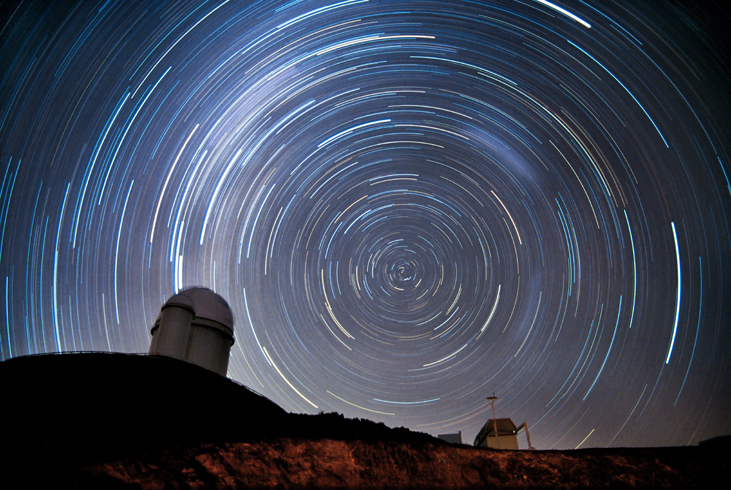
\includegraphics[width=0.5\textwidth]{Figures/Figure2.4.jpg}
\end{minipage}
\vspace{1em}


\question
The \fillin\ is defined as the period of 1 revolution of Earth around the Sun.

\begin{choices}
\correctchoice year
\choice day
\choice month
\choice week
\end{choices}

% \clearpage
\question
What does the blue line in the figure below represent?

\begin{figure}[h!]
    \centering
    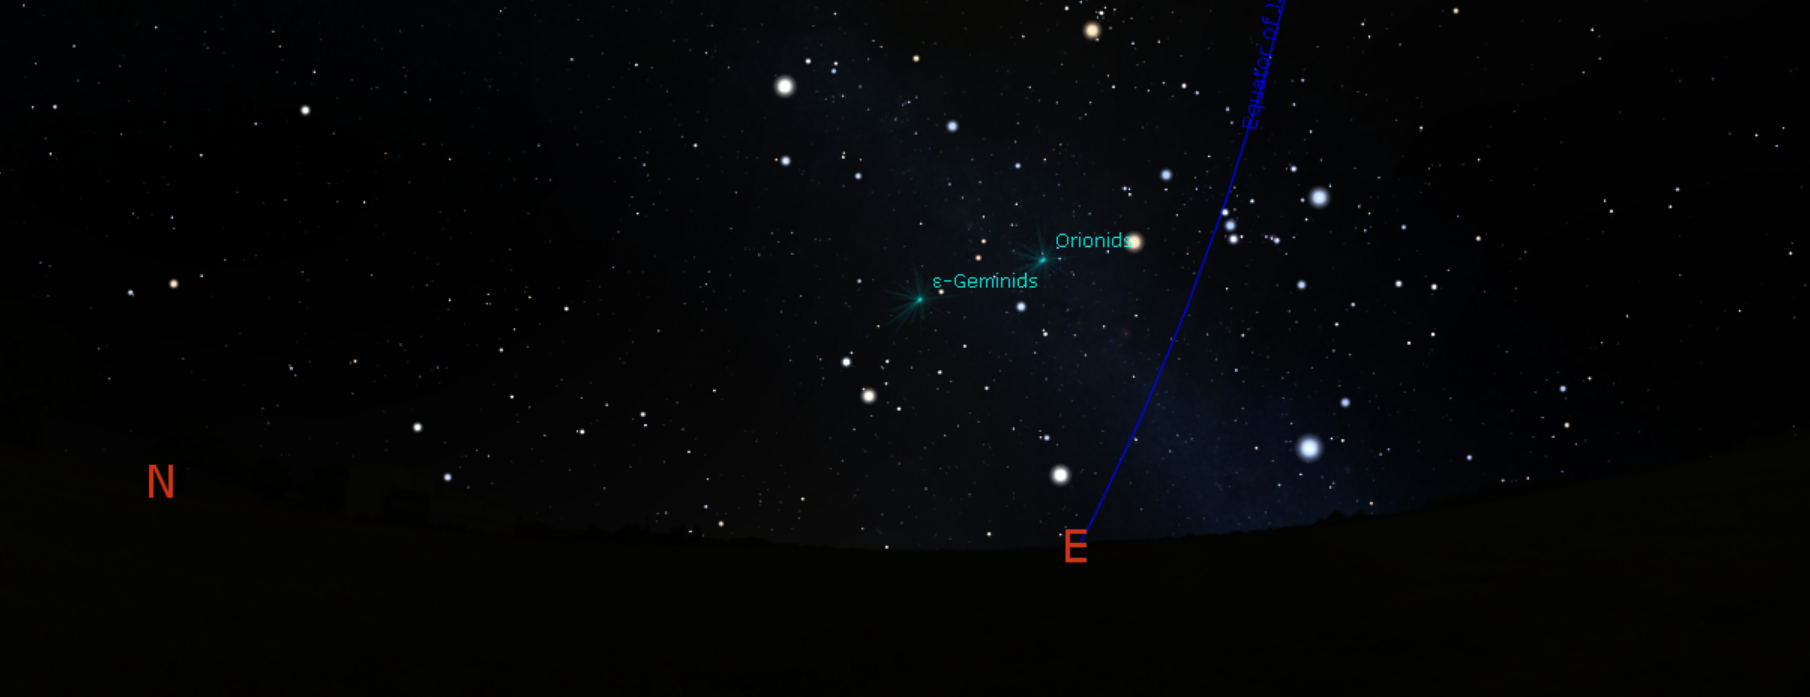
\includegraphics[width=4in]{Figures/Ch2_Fig_CelestialEquator.png}
    % \caption{Caption}
    % \label{fig:my_label}
\end{figure}

\begin{choices}
    \choice the ecliptic
    \correctchoice the celestial equator
    \choice the geographical equator
    \choice the zodiac
\end{choices}

\question
The celestial equator divides the celestial sphere into\dots.

\begin{choices}
    \correctchoice 2 northern and southern halves
    \choice 13 constellations of the zodiac
    \choice 4 caridnal directions (N, S, E, W)
    \choice 365 days of the year
\end{choices}

\question
The Sun's path on the celestial sphere across the calendar year is called the \fillin\ .

\begin{choices}
\choice zodiac
\choice constellation
\choice solar path
\correctchoice ecliptic
\end{choices}

\question
The 13 constellations of the zodiac are aligned with \fillin \ .

\begin{minipage}{0.3\textwidth}
    \centering
    \begin{choices}
    \choice the north celestial pole
    \correctchoice the ecliptic
    \choice the zenith
    \choice the solar eclipse
    \end{choices}
\end{minipage}%
\begin{minipage}{0.6\textwidth}
    \centering
    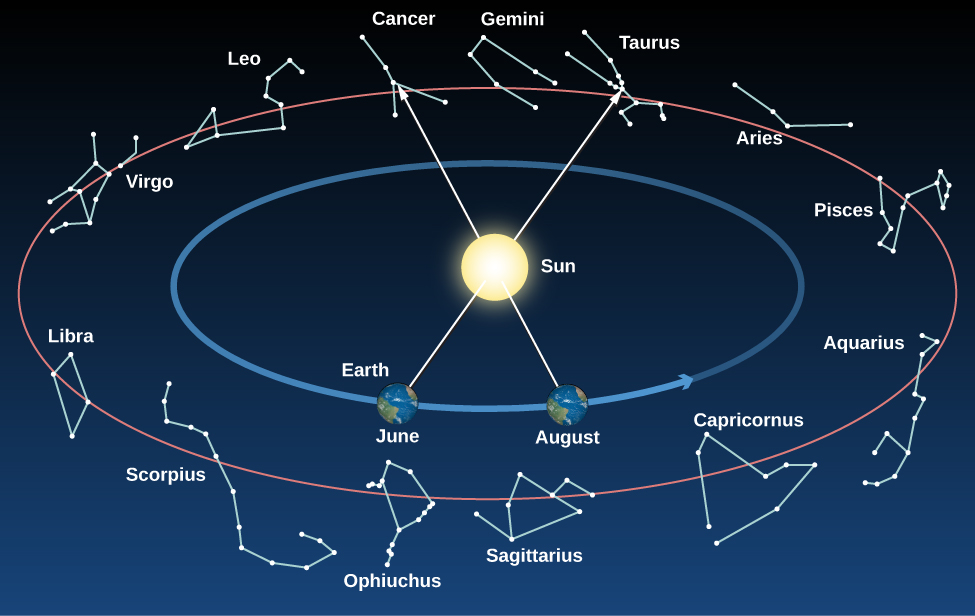
\includegraphics[width=0.5\textwidth]{Figures/Figure2.6.jpg}
\end{minipage}
\vspace{1em}

\question
What is the tilt of the celestial equator relative to the ecliptic?

\begin{minipage}{0.3\textwidth}
    \centering
    \begin{choices}
    \choice \SI{0.01}{\degree} 
    \choice \SI{30.0}{\degree} 
    \correctchoice \SI{23.5}{\degree} 
    \choice \SI{45.0}{\degree} 
    \end{choices}
\end{minipage}%
\begin{minipage}{0.6\textwidth}
    \centering
\scalebox{0.8}{
\centering
\begin{tikzpicture}

\def\R{3} % sphere radius
\def\angEl{23} % elevation angle
\def\angTilt{30} %tilt angle increased from 23.5 for emphasis

\pgfmathsetmacro\H{\R*cos(\angEl)} % distance to north pole
\draw (0,0) -- (0,\H*1.25);
\fill[yellow] (0.3,1.15) circle (3pt);
\draw[very thick] (0.3,1.15) circle (3pt);% node[above right] {\textbf{September}};

\begin{scope}[rotate=-\angTilt]
    \draw[very thin] (0,\H) -- (0,0);
\end{scope}
\shade[ball color=white, opacity=0.5] (0,0) circle (\R);
\coordinate[mark coordinate] (O) at (0,0);

\begin{scope}[rotate=-\angTilt]
    \DrawLatitudeCircleBack[\R]{0}
\end{scope}

\begin{scope}[rotate=-\angTilt]
        \DrawLatitudeCircleFront[\R]{0}
        \draw[thick] (0,\H*1.25) -- (0,\H) (0,0) -- (0,-1);
        \draw[very thick,blue,fill=white] (0,0) circle (19pt) node {\rotatebox{-\angTilt}{\textbf{Earth}}};
        \node at (0.2,0.9) {\textbf{N}};
        \node at (-0.2,-0.9) {\textbf{S}};
\end{scope}

\DrawLatitudeCircle[\R]{0}
\draw (-2,-0.9) --++ (-1.3,-0.6) node[below] {Ecliptic};

\fill[yellow] (-\R,0) circle (4pt); 
\draw[very thick] (-\R,0) circle (4pt);% node[left=7pt] {\textbf{December}};

\fill[yellow] (\R,0) circle (4pt);
\draw[very thick] (\R,0) circle (4pt);% node[right=6pt] {\textbf{June}};

\fill[yellow] (-0.3,-1.15) circle (4pt); 
\draw[very thick] (-0.3,-1.15) circle (4pt);% node[below=8pt] {\textbf{March}};

\draw[very thick,<->] (0,2.3) arc (90:55:1.85);
\node at (0.75,2.55) {tilt?};

\draw (1.7,-1.8) -- ++(1,-0.4) node[right] {Celestial Equator};

\draw[very thick,<->] (1.7,-1) arc (-10:-45:1.4);
\node at (2.1,-1.45) {\small {tilt?}};

\node at (-2.8,2.8) {Celestial Sphere};

\end{tikzpicture}
}
\end{minipage}
\vspace{1em}

\question
What is a planet?

\begin{choices}
\choice the stars that orbit the Sun
\choice spherical gas clouds on Earth
\correctchoice any of the 8 large bodies (including Earth) that orbit the Sun
\choice the Moon
\end{choices}

% \question
% Apparent magnitude is related to
% \fillin[][1in]\ .

% \begin{choices}
% \choice the distance to a star
% \choice the diameter of a planet
% \correctchoice how bright a star looks in the sky
% \choice the mass of the Sun
% \end{choices}


\question
If a model is \textit{heliocentric}, then it is \fillin\ .

\begin{choices}
\choice centered on Earth
\correctchoice centered on the Sun
\choice centered on the Moon
\choice ancient in origin
\end{choices}

\clearpage
% \section*{2.2 Ancient Astronomy}
% \subsection*{Early Greek and Roman Cosmology}

\question
Which shapes did Pythagoras believe to be ``perfect forms''?

\begin{choices}
    \choice hexagon
    \choice rhombus \& rectangle
    \choice ellipse
    \correctchoice circle \& sphere
\end{choices}

\question
Why did ancient Greeks like Pythagoras believe the gods prefer spheres?

\begin{choices}
    \choice the gods spoke to Pythagoras
    \choice the human head is shaped like a sphere (ball)
    \choice the gods actually preferred triangles
    \correctchoice the Sun and Moon are round and spherical
\end{choices}

\question
Which astronomical event did Aristotle reference to prove that the Sun must be farther away from us than the Moon?

\begin{choices}
    \choice a lunar eclipse
    \choice the sun rise
    \correctchoice a solar eclipse
    \choice the blue moon
\end{choices}

\question
Which of the following is NOT in agreement with Aristotle's arguments for a round Earth?

\begin{choices}
    \choice People in South America can see stars that are not visible in Texas.
    \choice The North Star looks lower in the sky in Florida than it does in Maine.
    \correctchoice The celestial sphere does not change when you geographically travel southward. 
    \choice Earth casts a round shadow on the Moon during a lunar eclipse.
\end{choices}


% \subsection*{Ptolemy's Model of the Solar System}

\question
Ptolemy's book, which served as the authority of astronomical knowledge for over 1400 years, was called the \fillin[\textit{Almagest}].

\begin{choices}
    \choice \textit{Principia Mathematica}
    \correctchoice \textit{Almagest}
    \choice \textit{On The Revolutions of Celestial Orbs}
    \choice \textit{Harry Potter and the Chamber of Secrets}
\end{choices}

\question
The purpose of Ptolemy's geometric model of the solar system was to \fillin\ .

\begin{choices}
    \choice prove that the solar system is geocentric
    \choice create the 12 constellations of the zodiac
    \correctchoice predict the positions of the Sun and planets at any date and time
    \choice prove that the solar system is heliocentric
\end{choices}

\question
True or False? Ptolemy's geocentric model was remarkable because it was simple and symmetrical.

\begin{choices}
    \choice True
    \correctchoice False
\end{choices}

% \clearpage
% \section*{2.4 The Birth of Modern Astronomy}

\question
What was Copernicus's motivation for challenging Ptolemy's model of the solar system?

\begin{choices}
    \choice He hated Ptolemy
    \correctchoice He wanted a better, simpler theory to predict where the planets will move in the sky
    \choice He wanted to prove that the geocentric model of the solar system was correct.
    \choice He actually agreed with Ptolemy's model.
\end{choices}

\question
What does ``heliocentric'' mean?

\begin{choices}
    \choice centered on the Earth
    \choice centered on the Moon
    \choice centered on Mars
    \correctchoice centered on the Sun
\end{choices}

\question
True or false? Ptolemy believed in a \textit{heliocentric} solar system, and Copernicus in a \textit{geocentric} one.

\begin{choices}
    \choice True
    \correctchoice False
\end{choices}

\question
According to Copernicus, the celestial sphere appears to rotate because\ldots\ .

\begin{choices}
    \correctchoice the Earth rotates on its axis (once every 24 hours)
    \choice the Sun is the center of the solar system
    \choice the universe revolves around the Earth
    \choice the atmosphere creates a rotational effect
    
\end{choices}

\question
Copernicus published his main book on the year he died, in \fillin\ .

\begin{choices}
    \correctchoice 1543
    \choice 1609
    \choice 140
    \choice 1492
\end{choices}

\clearpage

% \subsection*{Galileo}
\question
True to False? Copernicus proved beyond doubt that Earth and the planets revolve around the Sun.

\begin{choices}
    \choice True
    \correctchoice False
\end{choices}

\question
True or False? Galileo was a supporter of the Copernican (sun-centered) view of the universe.

\begin{choices}
    \correctchoice True
    \choice False
\end{choices}

\question
What is the significance of the discovery of Jupiter's 4 moons?

\begin{choices}
    \choice It proved that the solar system is Earth-centered.
    \choice It motivated Galileo to search the Milky Way for other faint objects.
    \choice It supported the Church's stance on a heliocentric universe.
    \correctchoice It was clear evidence that not everything revolves around Earth.
\end{choices}

\question
After Galileo, Earth was \ldots

\begin{choices}
    \choice proven to be a round object
    \correctchoice no longer considered the center of the universe
    \choice considered to have 3 more moons
    \choice hit by an asteroid
\end{choices}

\question
Did Galileo face consequences for his astronomical observations?

\begin{choices}
    \choice No. He was hailed a hero.
    \choice No. No one cared about his experiments.
    \correctchoice Yes. He was put under house arrest. 
    \choice Yes. He was executed.
\end{choices}

\end{questions}
\end{document}

% \question %3 
% Explain, according to both geocentric and heliocentric cosmologies, why we see retrograde motion of the planets.

% \question %6 
% Explain the origin of the magnitude designation for determining the brightness of stars. Why does it seem to go backward, with smaller numbers indicating brighter stars?

% \question %7 
% Ursa Minor contains the pole star, Polaris, and the asterism known as the Little Dipper. From most locations in the Northern Hemisphere, all of the stars in Ursa Minor are circumpolar. Does that mean these stars are also above the horizon during the day? Explain.

% \question %9 
% How many degrees does the Moon move per day relative to the fixed stars? How many days does it take for the Moon to return to its original location relative to the fixed stars?


% \question %11 
% The Sun was once thought to be a planet. Explain why.

% \question %13 
% What is an asterism? Can you name an example?

% \question %17 
% How did Hipparchus discover the wobble of Earth's axis, known as precession?

% \question %18 
% Why did Ptolemy have to introduce multiple circles of motion for the planets instead of a single, simple circle to represent the planet's motion around the Earth?

% \question %21 
% What phases would Venus show if the geocentric model were correct?

\question %24. 
% Draw a picture that explains why Venus goes through phases the way the Moon does, according to the heliocentric cosmology. Does Jupiter also go through phases as seen from Earth? Why?

% \question %25. 
% Show with a simple diagram how the lower parts of a ship disappear first as it sails away from you on a spherical Earth. Use the same diagram to show why lookouts on old sailing ships could see farther from the masthead than from the deck. Would there be any advantage to posting lookouts on the mast if Earth were flat? (Note that these nautical arguments for a spherical Earth were quite familiar to Columbus and other mariners of his time.)

% \question %26. 
% Parallaxes of stars were not observed by ancient astronomers. How can this fact be reconciled with the heliocentric hypothesis?

% \question %27. 
% Why do you think so many people still believe in astrology and spend money on it? What psychological needs does such a belief system satisfy?

% \question %28. 
% Consider three cosmological perspectives---the geocentric perspective, the heliocentric perspective, and the modern perspective---in which the Sun is a minor star on the outskirts of one galaxy among billions. Discuss some of the cultural and philosophical implications of each point of view.

% \question %29. 
% The north celestial pole appears at an altitude above the horizon that is equal to the observer's latitude. Identify Polaris, the North Star, which lies very close to the north celestial pole. Measure its altitude. (This can be done with a protractor. Alternatively, your fist, extended at arm's length, spans a distance approximately equal to 10°.) Compare this estimate with your latitude. (Note that this experiment cannot be performed easily in the Southern Hemisphere because Polaris itself is not visible in the south and no bright star is located near the south celestial pole.)

% \question %30. 
% What were two arguments or lines of evidence in support of the geocentric model?

% \question %31. 
% Although the Copernican system was largely correct to place the Sun at the center of all planetary motion, the model still gave inaccurate predictions for planetary positions. Explain the flaw in the Copernican model that hindered its accuracy.

% \question %32. 
% During a retrograde loop of Mars, would you expect Mars to be brighter than usual in the sky, about average in brightness, or fainter than usual in the sky? Explain.

% \question %33. 
% The Great Pyramid of Giza was constructed nearly 5000 years ago. Within the pyramid, archaeologists discovered a shaft leading from the central chamber out of the pyramid, oriented for favorable viewing of the bright star Thuban at that time. Thinking about Earth's precession, explain why Thuban might have been an important star to the ancient Egyptians.

% \question %34. 
% Explain why more stars are circumpolar for observers at higher latitudes.

% \question %37. 
% Hipparchus could have warned us that the dates associated with each of the natal astrology sun signs would eventually be wrong. Explain why.

% \question %38. 
% Explain three lines of evidence that argue against the validity of astrology.

\question %41. 
% Suppose Eratosthenes had found that, in Alexandria, at noon on the first day of summer, the line to the Sun makes an angle \SI{30}{\degree} with the vertical. What, then, would he have found for Earth's circumference?

% \question %42. 
% Suppose Eratosthenes' results for Earth's circumference were quite accurate. If the diameter of Earth is 12,740 km, what is the length of his stadium in kilometers?